\chapter{Cyber Threat Intelligence}

In ambito di sicurezza, il concetto di \textit{Intelligence} si riferisce all'acquisizione 
e allo studio di informazioni strategiche riguardanti un potenziale avversario. 
Identificare l'identità dell'attaccante, comprenderne a fondo le motivazioni e 
valutarne le risorse a disposizione costituiscono operazioni complesse ma di 
fondamentale importanza. Affinché tale conoscenza risulti davvero efficace, è 
essenziale che le informazioni vengano raccolte ed elaborate in tempi rapidi, 
consentendo così la pianificazione e l'attuazione di adeguate contromisure difensive.

\section{Ecosistema della CTI}

Declinando questo approccio nel dominio informatico, si parla specificamente di 
\textbf{Cyber Threat Intelligence (CTI)}. In questo contesto, è cruciale tracciare 
una netta distinzione tra il semplice "dato" e l'"intelligence" vera e propria. 
Quest'ultima non può basarsi sulla mera raccolta di dati grezzi, i quali necessitano 
obbligatoriamente di un processo di analisi, elaborazione e contestualizzazione. A 
titolo esemplificativo, il semplice rilevamento di un \textit{data leak} non 
costituisce di per sé intelligence; lo diventa nel momento in cui tali informazioni 
vengono incrociate e correlate con ulteriori dettagli specifici, permettendo di 
delineare un quadro della minaccia chiaro e utilizzabile a fini difensivi.

Tipi di CTI:

\begin{itemize}
    \item \textbf{Strategica}: Rivolta al \textit{C-level} (personale manageriale), 
    focalizzata su trend e allocazione di risorse a lungo termine.
    \item \textbf{Operativa}: Per gli \textit{Incident Responder} di alto livello. Risponde a
    domande sul "\textit{chi?}", "\textit{perché?}" e valuta campagne specifiche.
    \item \textbf{Tattica}: A brevissimo termine, usata dai team SOC. Si basa su 
    artefatti di rete, IP, domini e hash.
\end{itemize}

Esempio dei \textit{Conti Leaks}: i \textbf{Conti Leaks}, definiti i "\textit{Panama Papers del 
ransomware}", sono un esempio magistrale di CTI operativa derivata da un leak interno. 
L'analisi di questi dati ha permesso di scoprire che il gruppo Conti operava come una 
vera e propria azienda legittima, con dipartimenti HR, tester, reverser, team OSINT e 
persino personale dedicato al training. Ha inoltre rivelato le connessioni operative 
con altri gruppi (\textit{Revil}) e malware (\textit{Ryuk}, \textit{Maze}).

\section{Dati e IOC}

Le fonti informative ("\textit{INTs}") nutrono la CTI. Le principali includono:

\begin{itemize}
    \item \textbf{OSINT (Open-Source Intelligence)}: Dati pubblici, reportistica, 
    query WHOIS o record DNS.
    \item \textbf{HUMINT (Human Intelligence)}: Informazioni derivanti da interazioni 
    umane, come interviste a soggetti coinvolti in intrusioni o leak diretti dai 
    threat actor.
    \item \textbf{Deep/Dark Web e Honeypot}: Sistemi civetta configurati per emulare
    macchine reali e catturare tentativi di exploit o payload di malware.
\end{itemize}

Gli \textbf{Indicatori di Compromissione (IOC)} sono evidenze forensi lasciate 
dall'attaccante (qualsiasi informazione di basso livello di rete o su log). A tal 
proposito riportiamo l'esempio reale del ransomware \textit{Bad Rabbit}:

\begin{lstlisting}
Network/Host Artifacts:
- Domain: hxxp://caforssztxqzf2nm[.]onion 
- Domain: hxxp://argumentiru[.]com 
- IP: 185.149.120[.]3 
- Hash (SHA-1): de5c8d858e6e41da715dca1c019df0bfb92d32c0 
\end{lstlisting}

L'analisi di tali informazioni ha portato a scoprire l'URL che il gruppo di hacker ha usato per 
trasferire il riscatto, il sito di notizie russo infettato con il malware stesso e l'hash 
del payload. L'hash che vediamo è a tutti gli effetti un'impronta digitale, si tratta 
magari dell'hash di un eseguibile che è stato già etichettato come malevolo. L'antivirus stesso 
conserva nel proprio DB solo l'hash dei malware perchè è più pratico e leggero da conservare dato 
che sono appena 64 byte.

Perché usiamo file hash e domini? E perché a volte falliscono? La risposta risiede 
nella \textbf{Pyramid of Pain} di David J. Bianco. Questa piramide modella lo sforzo 
richiesto all'attaccante se il difensore blocca un indicatore:

\begin{figure}[H]
    \centering
    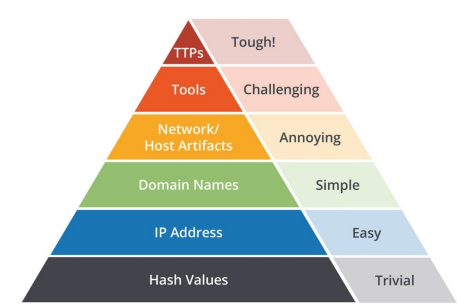
\includegraphics[width=0.6\linewidth]{img/capitolo9/pyramid.png}
    \label{fig:pyramid}
\end{figure}

\begin{enumerate}
    \item \textbf{Hash Values (Trivial)}: Bannare l'hash di Bad Rabbit è banale, per 
    l'attaccante basta alterare un singolo bit nel payload (es. recompilando o 
    aggiungendo un byte nullo) per cambiare totalmente l'hash, vanificando la difesa.
    \item \textbf{IP/Domini (Easy/Simple)}: L'attaccante usa tecniche di \textit{Fast Flux} 
    o DGA (\textit{Domain Generation Algorithms}) per cambiare rapidamente infrastruttura.
    \item \textbf{TTPs - Tactics, Techniques, and Procedures (Tough)}: Bloccare una 
    TTP (es. bloccare le esecuzioni di \textit{PowerShell} non firmate) costringe 
    l'attaccante a dover riscrivere i tool e cambiare le proprie procedure operative. 
    È qui che la difesa ha il massimo impatto.
\end{enumerate}

\section{Piattaforme e Standard}

Nel contesto operativo della Cyber Threat Intelligence, l'analisi, la catalogazione e 
la condivisione delle informazioni si avvalgono di strumenti e piattaforme specifiche, 
fondamentali per contrastare le minacce in modo tempestivo.

Tra gli strumenti di analisi tecnica spicca \textbf{VirusTotal}, un servizio che 
consente di scansionare file eseguibili tramite l'upload diretto sulla piattaforma. 
Il sistema è progettato per ottimizzare i tempi di risposta: qualora l'eseguibile 
sia già presente nel database e precedentemente analizzato, i risultati vengono 
restituiti quasi istantaneamente. In caso di file inediti, invece, il sistema avvia 
autonomamente un'analisi approfondita avvalendosi di molteplici motori antivirus.

Un approccio complementare è offerto da \textbf{AlienVault}, che opera come un vero e 
proprio aggregatore di informazioni sulle minacce. Rispetto a VirusTotal, questa 
piattaforma si distingue per una natura spiccatamente più "\textit{social}" e 
collaborativa. Caricando un malware al suo interno, il sistema non si limita ad 
analizzarlo, ma è in grado di correlarlo ad altre minacce, permettendo agli analisti 
di individuare pattern ricorrenti e, in molti casi, di ricondurre attacchi 
apparentemente isolati a una medesima entità attaccante.

Spostandoci su una dimensione più strutturata e aziendale, l'esigenza di monitorare 
minacce altamente specifiche per il proprio settore operativo come, ad esempio, il 
comparto bancario richiede l'impiego delle \textbf{Threat Intelligence Platform (TIP)}. 
In questo ecosistema, la soluzione open source di maggiore rilevanza, nonché la più 
adottata a livello europeo, è \textbf{MISP} (\textit{Malware Information Sharing Platform}). 
Tale piattaforma permette di creare archivi dettagliati e pagine specifiche per ogni 
evento o minaccia rilevata, facilitando l'analisi interna.

Tuttavia, affinché questa vasta mole di intelligence possa essere scambiata 
efficacemente tra diverse organizzazioni, è imperativo l'utilizzo di standard 
universali per la rappresentazione e la trasmissione dei dati. I due protocolli di 
riferimento a livello globale sono STIX e TAXII:

\begin{itemize}
    \item \textbf{STIX}: rappresenta il modello linguistico e lo schema relazionale. 
    Esso definisce un'architettura standardizzata, basata su formato JSON, che 
    stabilisce esattamente quali informazioni raccogliere e come strutturare i 
    dettagli tecnici delle minacce.
    \item \textbf{TAXII}: costituisce invece lo standard per il trasporto di questi 
    dati. È un protocollo di comunicazione che permette di configurare in modo 
    granulare la distribuzione dell'intelligence, consentendo lo scambio di 
    informazioni su larga scala o limitandone la diffusione a specifici gruppi 
    ristretti e reti di fiducia.
\end{itemize}

\subsection{Threat Intelligence Feeds}

Un'organizzazione non è necessariamente tenuta a sviluppare e mantenere una funzione 
di Threat Intelligence esclusivamente all'interno del proprio organico. Spesso, per 
ragioni di costi o competenze, risulta strategico affidarsi a servizi commerciali 
forniti da vendor specializzati esterni (modello \textit{Intelligence as a Service}). 
Un esempio emblematico in questo settore è rappresentato dalla piattaforma 
\textbf{Digital Shadows}.

Questo tipo di soluzioni commerciali offre un monitoraggio completo e altamente 
contestualizzato del panorama cibernetico. La piattaforma fornisce un aggiornamento 
continuo attraverso feed informativi sugli attacchi andati a buon fine a livello 
globale, elabora reportistica di dettaglio e, soprattutto, produce sintesi mirate 
che evidenziano quali specifiche minacce potrebbero colpire i diretti \textit{asset} 
dell'azienda cliente.

Il valore aggiunto di tali strumenti risiede in particolare in due funzionalità 
analitiche e di monitoraggio avanzate:

\begin{itemize}
    \item \textbf{Correlazione delle vulnerabilità}: Il sistema è in grado di 
    incrociare in modo proattivo le debolezze e le vulnerabilità note presenti 
    nell'infrastruttura dell'azienda con quelle che vengono attivamente sfruttate 
    (o "armate") dagli attaccanti \textit{in the wild}. Questa contestualizzazione 
    permette ai team di sicurezza di stabilire priorità d'intervento precise per il 
    \textit{patch management}, concentrandosi sui rischi reali ed imminenti.
    \item \textbf{Monitoraggio del Dark Web}: La piattaforma effettua una 
    sorveglianza continua delle reti sommerse e dei forum underground. Qualora dati 
    sensibili, credenziali compromesse o informazioni riservate riconducibili 
    all'organizzazione dovessero emergere in questi ambienti (ad esempio a seguito di 
    una fuga di dati di terze parti), il sistema genera alert tempestivi, consentendo 
    all'azienda di attuare misure di contenimento preventive prima che tali dati 
    vengano sfruttati in attacchi diretti.
\end{itemize}

\section{Framework Analitici}

Modellare e rappresentare in modo accurato una tecnica di attacco è un'operazione 
intrinsecamente complessa. Per superare questa sfida e standardizzare il linguaggio 
utilizzato dagli analisti, l'industria della sicurezza informatica ha sviluppato 
specifici framework di riferimento. I tre modelli principali utilizzati nella Threat 
Intelligence sono la \textbf{Cyber Kill Chain}, il \textbf{Diamond Model} e il 
framework \textbf{MITRE ATT\&CK}.

\subsection{Cyber Kill Chain}

Sviluppato originariamente da Lockheed Martin, questo modello concettuale descrive 
l'anatomia di un attacco informatico suddividendolo in 7 fasi sequenziali. Assegnando 
un nome e una funzione a ciascun passaggio (come la \textit{Reconnaissance} o 
ricognizione, la \textit{Weaponization} o armamento, fino all'azione sugli obiettivi), 
il framework permette ai difensori di tracciare la progressione della minaccia con 
l'obiettivo di "spezzare la catena" prima che l'attacco venga portato a termine.

\begin{figure}[H]
    \centering
    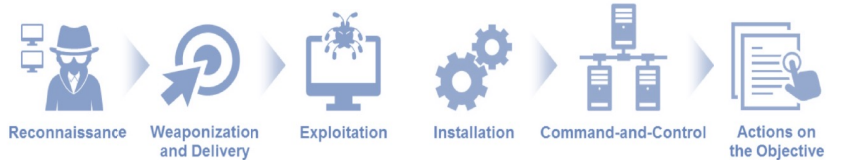
\includegraphics[width=1\linewidth]{img/capitolo9/ckc.png}
    \label{fig:ckc}
\end{figure}

\subsection{Diamond Model}

Il Diamond Model è uno standard di analisi di alto livello progettato per modellare 
le intrusioni evidenziando le relazioni logiche alla base di un incidente di 
sicurezza.

\begin{figure}[H]
    \centering
    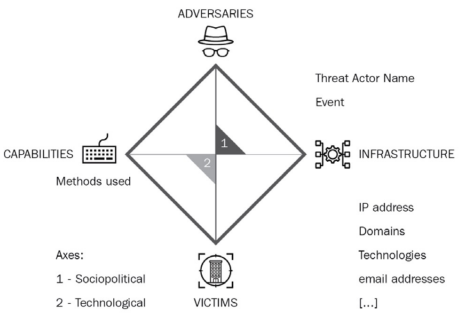
\includegraphics[width=0.7\linewidth]{img/capitolo9/diamond.png}
    \label{fig:diamond}
\end{figure}

Visivamente rappresentato come un rombo, il modello si fonda su quattro elementi 
(o vertici) interconnessi:

\begin{itemize}
    \item \textbf{L'Avversario}: L'identità o il gruppo che orchestra l'attacco 
    (es. un gruppo State-sponsored o un'organizzazione criminale).
    \item \textbf{La Vittima}: Il bersaglio dell'offensiva, che può essere 
    un'infrastruttura, un'azienda o uno specifico asset.
    \item \textbf{Le Capacità}: Gli strumenti, le tecniche e le competenze tecniche 
    a disposizione dell'attaccante.
    \item \textbf{L'Infrastruttura}: Le risorse fisiche o logiche utilizzate per 
    veicolare l'attacco.
\end{itemize}

\subsection{MITRE ATT\&CK}

Sviluppato dal MITRE, l'ATT\&CK è la base di conoscenza globale più autorevole e 
comprensiva sulle metodologie di attacco. Essendo in continuo aggiornamento, ogni 
qualvolta viene scoperta una nuova metodologia offensiva \textit{in the wild}, il 
catalogo viene espanso. Sebbene la matrice principale sia focalizzata sugli ambienti 
aziendali (\textit{Enterprise}), esistono schemi dedicati anche ad altri domini, 
come il \textit{Cloud}, i dispositivi mobili e i sistemi di controllo industriale 
(\textit{ICS}).

L'architettura logica del MITRE ATT\&CK è organizzata sotto forma di matrice e si 
articola in una gerarchia di tre livelli:

\begin{figure}[H]
    \centering
    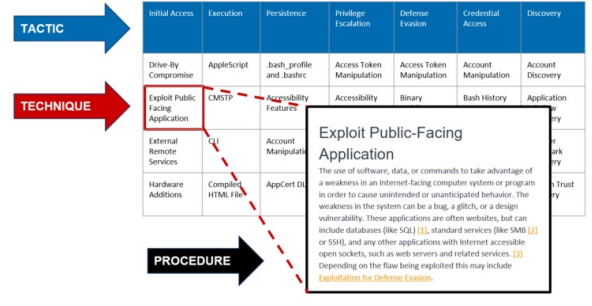
\includegraphics[width=1\linewidth]{img/capitolo9/mitre.png}
    \label{fig:mitre}
\end{figure}

\begin{itemize}
    \item \textbf{Tattiche (Tactics)}: Rappresentano l'obiettivo strategico o il 
    motivo per cui un'azione viene compiuta (il "\textit{perché}"). Nella matrice, 
    le tattiche costituiscono le intestazioni delle colonne.
    \item \textbf{Tecniche (Techniques)}: Descrivono il metodo specifico utilizzato 
    per raggiungere una determinata tattica (il "\textit{come}"). All'interno di ogni 
    colonna si trovano le diverse tecniche associate a quell'obiettivo.
    \item \textbf{Procedure (Procedures)}: Costituiscono l'implementazione pratica e 
    specifica della tecnica. Poiché sistemi diversi richiedono approcci diversi, 
    l'esecuzione di una medesima tecnica su un ambiente Windows piuttosto che su 
    macOS richiederà l'uso di procedure e porzioni di codice profondamente distinte.
\end{itemize}

Infine, il framework MITRE non si limita alla classificazione offensiva ma possiede 
un forte valore difensivo: per ogni tecnica censita, la piattaforma fornisce 
informazioni cruciali sulle contromisure preventive e suggerisce regole di \textit{detection}, 
offrendo spunti su come implementare porzioni di codice e configurazioni per rilevare 
la minaccia all'interno della propria infrastruttura.